\documentclass{article}
\usepackage[utf8]{inputenc}
\usepackage{hyperref}
\usepackage{graphicx}
\usepackage{float}
\usepackage{listings}
\setlength{\parindent}{0em}
\setlength{\parskip}{1em}

\title{New Devices Lab: smart wall hangers}
\author{Elina Antonova \quad \\ Maikel Jans \quad}
\date{\today}

\begin{document}

\maketitle

\tableofcontents

\newpage

\section{Introduction}
For our New Devices Lab project we are making smart wall hangers. The goal of this product is to make it easier to see at a glance what a user should take with them on the coming trip. For example, our wall hanger reminds the user before going out that they should take their wallet with them. There are several other categories to choose from. The wall hanger should be customizable and modular. Wall hangers also have a notification system, which plays music in specified time, check out system and web/mobile application support.

\section{Design}
Each wall hanger has two hooks and two shelf sections. Hooks are modelled for things that are possible to hang, while shelf sections are made for things such as power bank, wallet, glasses, etc.

We have 9 predefined categories of the different things that can be placed on our wall hangers: keys, bag, bottle, glasses, headphones, coat, money (wallet), power bank, umbrella. The categories are predefined by us, because their logos and texts were specifically designed for the OLED screens that we are using. Every hook and shelf section have a corresponding OLED display, which are assigned with a category for the next trip, and they display a corresponding category's icon and text as a reminder of what user should be taking with them to their this trip. 

We have added an app support for the shelves. When user is logged in, wall hangers can be added to their account, edited and deleted. Each wall hanger (named \textit{shelf} in the app) has globally unique identifier and location, which can be added and edited by users. 

Users can also add, edit and delete future trips. For each trip they select their destination, start and end time, reminder time and customize each shelves' OLED screens with the corresponding categories they want to display. 

In addition, we are using NFC to make it possible for user to check out before the trip. We are using a speaker to notify the user when they need to leave if they have not checked out with their NFC tag yet. The NFC reader and the speaker are located only on one wall hanger in the set, which will be considered the "main" wall hanger. The wall hanger can be marked main through the app we are creating. 

We are using infrared (IR) sensors to detect when corresponding items were removed from the shelf/hook and we use front end to send a reminder of forgotten item. However, we had encountered time issue and only partially implemented this feature. 

We have the micro controller on every shelf that request data from the back end and, depending on the shelf settings of the closest trip, they set up what screens display, when the speaker should play a reminder music, update the IR obstacle sensor state in the back end, etc. 

\subsection{List of components}

In addition to 2 wood pieces for shelf sections and back panel wall hangers contain the following electronical components:
\begin{itemize}
    \item 1 ESP32 WROOM 4Mb Devkit V1 Board
    \item 1 I2C TCA9548A Multiplexer 
    \item 4 Mini 0.91 inch I2C OLED displays
    \item 6 infrared (IR) obstacle sensors 
    \item 1 RFID-RC522 NFC Kit (only on main shelf)
    \item 1 3W speaker (only on main shelf)
    \item PAM8403 5V Audio Amplifier (only on main shelf)
\end{itemize}

The shelf also contains some 3D printed details, that are discussed later in \hyperref[sec:mechanical]{Mechanical design} section. List of printed details: 

\begin{itemize}
    \item 2 hangers
    \item 2 screen holders
    \item 2 front side pieces for the shelf sections
    \item 2 back side pieces for the shelf sections
    \item 1 shelf sections separator 
\end{itemize}

\section{Mechanical Design}
\label{sec:mechanical}
For our project we mostly use wood, sensors and micro controllers. In addition to this we have created some 3D designs for our custom details. Figures 2 to 6 show details, where the top part and sides are open. This decision was been made on purpose to make wall hanger assembly easier and these details can be covered using printed rectangles of the same depth and width and glue. The workflow is not affected by missing covers and it was decided not to use more material on these parts. 

\subsection{Hook}
\hyperref[fig:hook]{Figure 1} shows the design of the hook. The image represents hook on its side, however, when placed on the wood it has the following dimensions: height - 72mm, depth - 60mm, width - 17 mm. This hook's design is similar to hooks used for coats, but we have added a small cube in the corner to make the hook sturdier, smaller hole is used to screw IR obstacle sensor to the hook and two big holes are used for attaching hook to the back panel using screws.
\begin{figure}[H]
    \begin{center}
        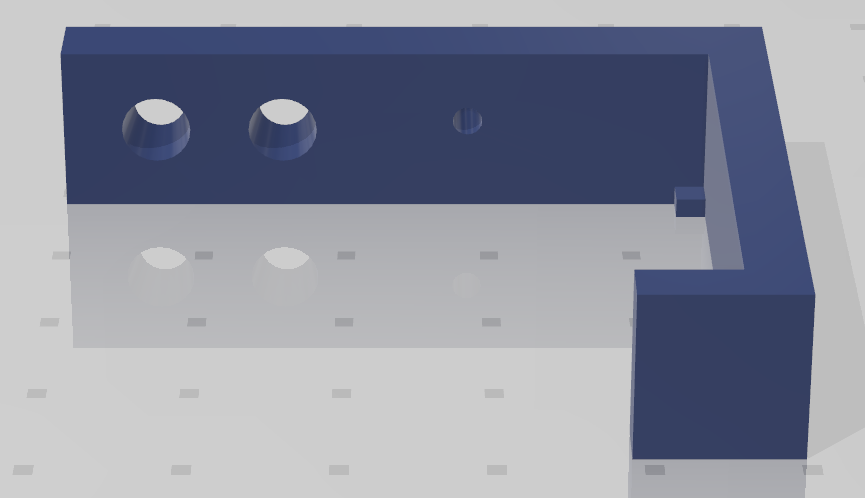
\includegraphics[width=0.7\textwidth]{3d/hook.png}
    \end{center}
    \caption{3D model of the hook}
    \label{fig:hook}
\end{figure}

\subsection{Screen holder}
\hyperref[fig:screen]{Figure 2} shows a 3D design of screen holders that are used to attach screens to the wood. It has the following dimensions: height - 14mm, depth - 23mm, width - 50 mm. The screen holders are open from the top, which makes screen assembly and replacement easier. The front part is used for the screen itself and the wall in the middle keeps it in place. The back part is used for attaching the holder to the wood and for hiding the wiring behind the shelf. Some decisions of this design are discussed by us later in \hyperref[sec:3dproblems]{3D models decisions problems} section.

\begin{figure}[H]
    \begin{center}
        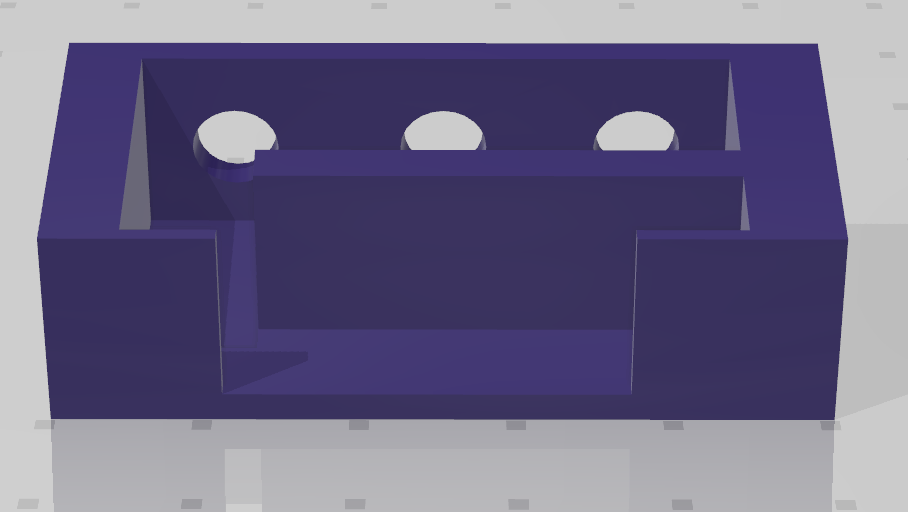
\includegraphics[width=0.7\textwidth]{3d/screen_holder.png}
    \end{center}
    \caption{3D model of the screen holder}
    \label{fig:screen}
\end{figure}

\subsection{Speaker holder}
\hyperref[fig:speaker]{Figure 3} shows a 3D design of speaker holder with the following dimensions: height - 46mm, depth - 29mm, width - 55 mm. The speaker is placed to the right part between the round hole and wall in the middle that is made to keep it in place. The left bottom corner is designed for amplifier. The back side is made for closing the box and the hole is designed for wires that connect amplifier to the microcontroller. The holder sizes are perfectly designed to place it at the back of the shelf breadth wise into 3D designed part shown in \hyperref[fig:shelf-back]{Figure 4}.
\begin{figure}[H]
    \begin{center}
        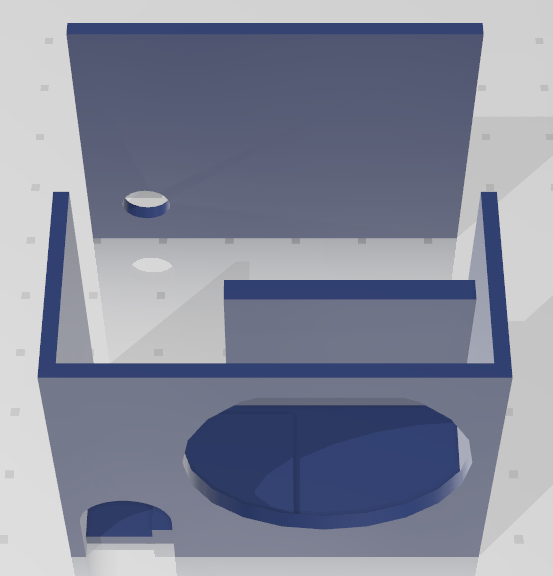
\includegraphics[width=0.5\textwidth]{3d/speaker.png}
    \end{center}
    \caption{3D model of the speaker holder}
    \label{fig:speaker}
\end{figure}

\subsection{Back side detail of the shelf}
\hyperref[fig:shelf-back]{Figure 4} represents a 3D design of the back side of the shelf section with dimensions: height - 30mm, depth - 60mm, width - 195 mm. It is used for IR obstacle sensors, wires and microcontroller. Two IR sensors are placed in the two rectangle holes to send/receive a signal. The two holes on the bottom are designed for screwing the sensors to the printed detail. However, the detail is placed straight on the shelf and these two bolt holes became unnecessary, since it is not possible to fit a nut under the printed detail. It is possible to use the holes if the detail will be placed 2-3 mm above the shelf. The round hole at the back is designed to bring the wires from the hooks/screen holders through the back of the shelf, but this decision was discussed by us in \hyperref[sec:3dproblems]{3D models decisions problems} section.
\begin{figure}[H]
    \begin{center}
        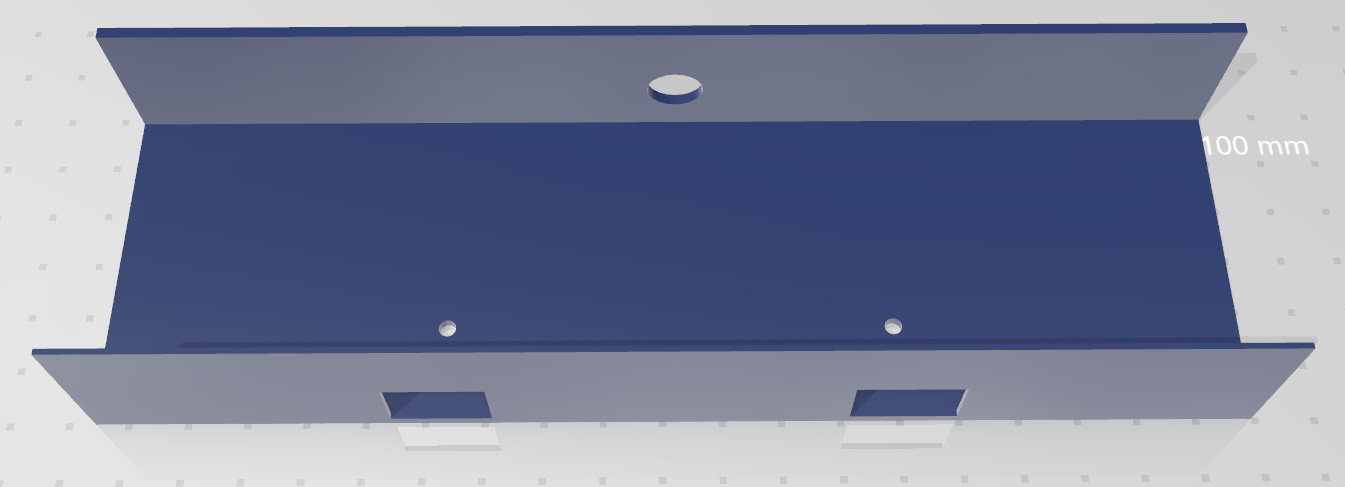
\includegraphics[width=\textwidth]{3d/shelf-back.png}
    \end{center}
    \caption{3D model of the back side of shelf section}
    \label{fig:shelf-back}
\end{figure}

\subsection{Front side detail of the shelf}
\hyperref[fig:shelf-front]{Figure 5} is a 3D design of the front side of the shelf section with the following dimensions: height - 30mm, depth - 30mm, width - 195 mm. The front part of the picture represents the back side of the detail and more complicated part is the (facing user) front part of the detail. The back side of it is used for reflecting the signal sent by IR obstacle sensors when no object is placed on the shelf section. The screen is placed in the middle of detail and design is similar to the one shown in \hyperref[fig:screen]{Figure 2}. NFC reader is placed only on the main shelf on one section and the top right holes and notches are designed for it. These holes and notches are absent on details that are not designed to have NFC reader on them (another part of main shelf and all extension shelves' sections). 

\begin{figure}[H]
    \begin{center}
        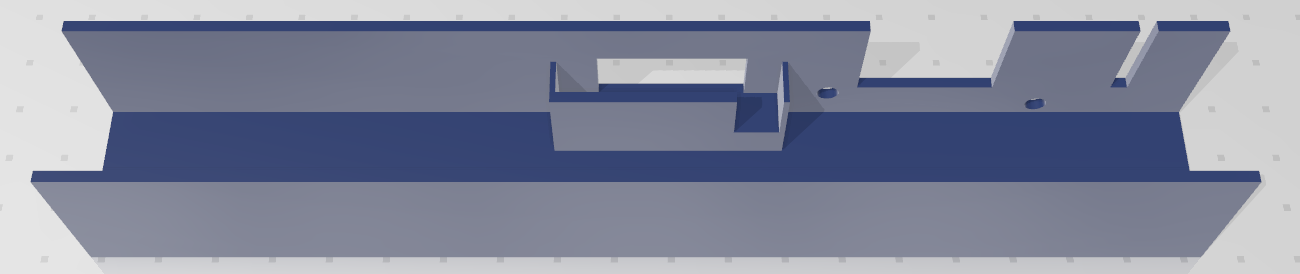
\includegraphics[width=\textwidth]{3d/shelf-front.png}
    \end{center}
    \caption{3D model of the front side of shelf section}
    \label{fig:shelf-front}
\end{figure}

\subsection{Shelf sections separator}
\hyperref[fig:shelf-separator]{Figure 6} is a 3D design of the shelf sections separation detail with the following dimensions: height - 30mm, depth - 200mm, width - 10 mm. The inner part is designed for connection of wires between screens and NFC located in the front part of the shelf and the microcontroller placed at the back of the shelf.

\begin{figure}[H]
    \begin{center}
        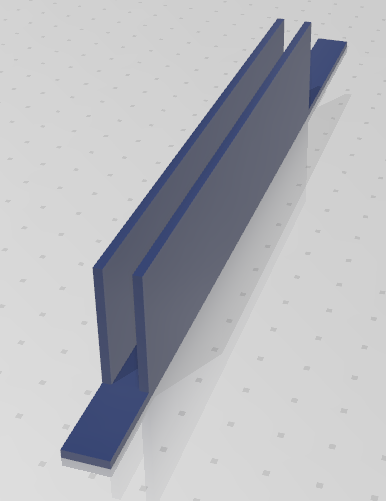
\includegraphics[width=0.4\textwidth]{3d/separation.png}
    \end{center}
    \caption{3D model of shelf sections separator}
    \label{fig:shelf-separator}
\end{figure}

\section{Electronic Design}
The components are not in the same layout as on a shelf, but the connections remain the same. The two figures \hyperref[fig:electronics-main]{Figure 7} and \hyperref[fig:electronics-extension]{Figure 8} represent the electronic designs of main and extension wall hangers. These images were made using the Fritzing application.
\begin{figure}[H]
    \begin{center}
        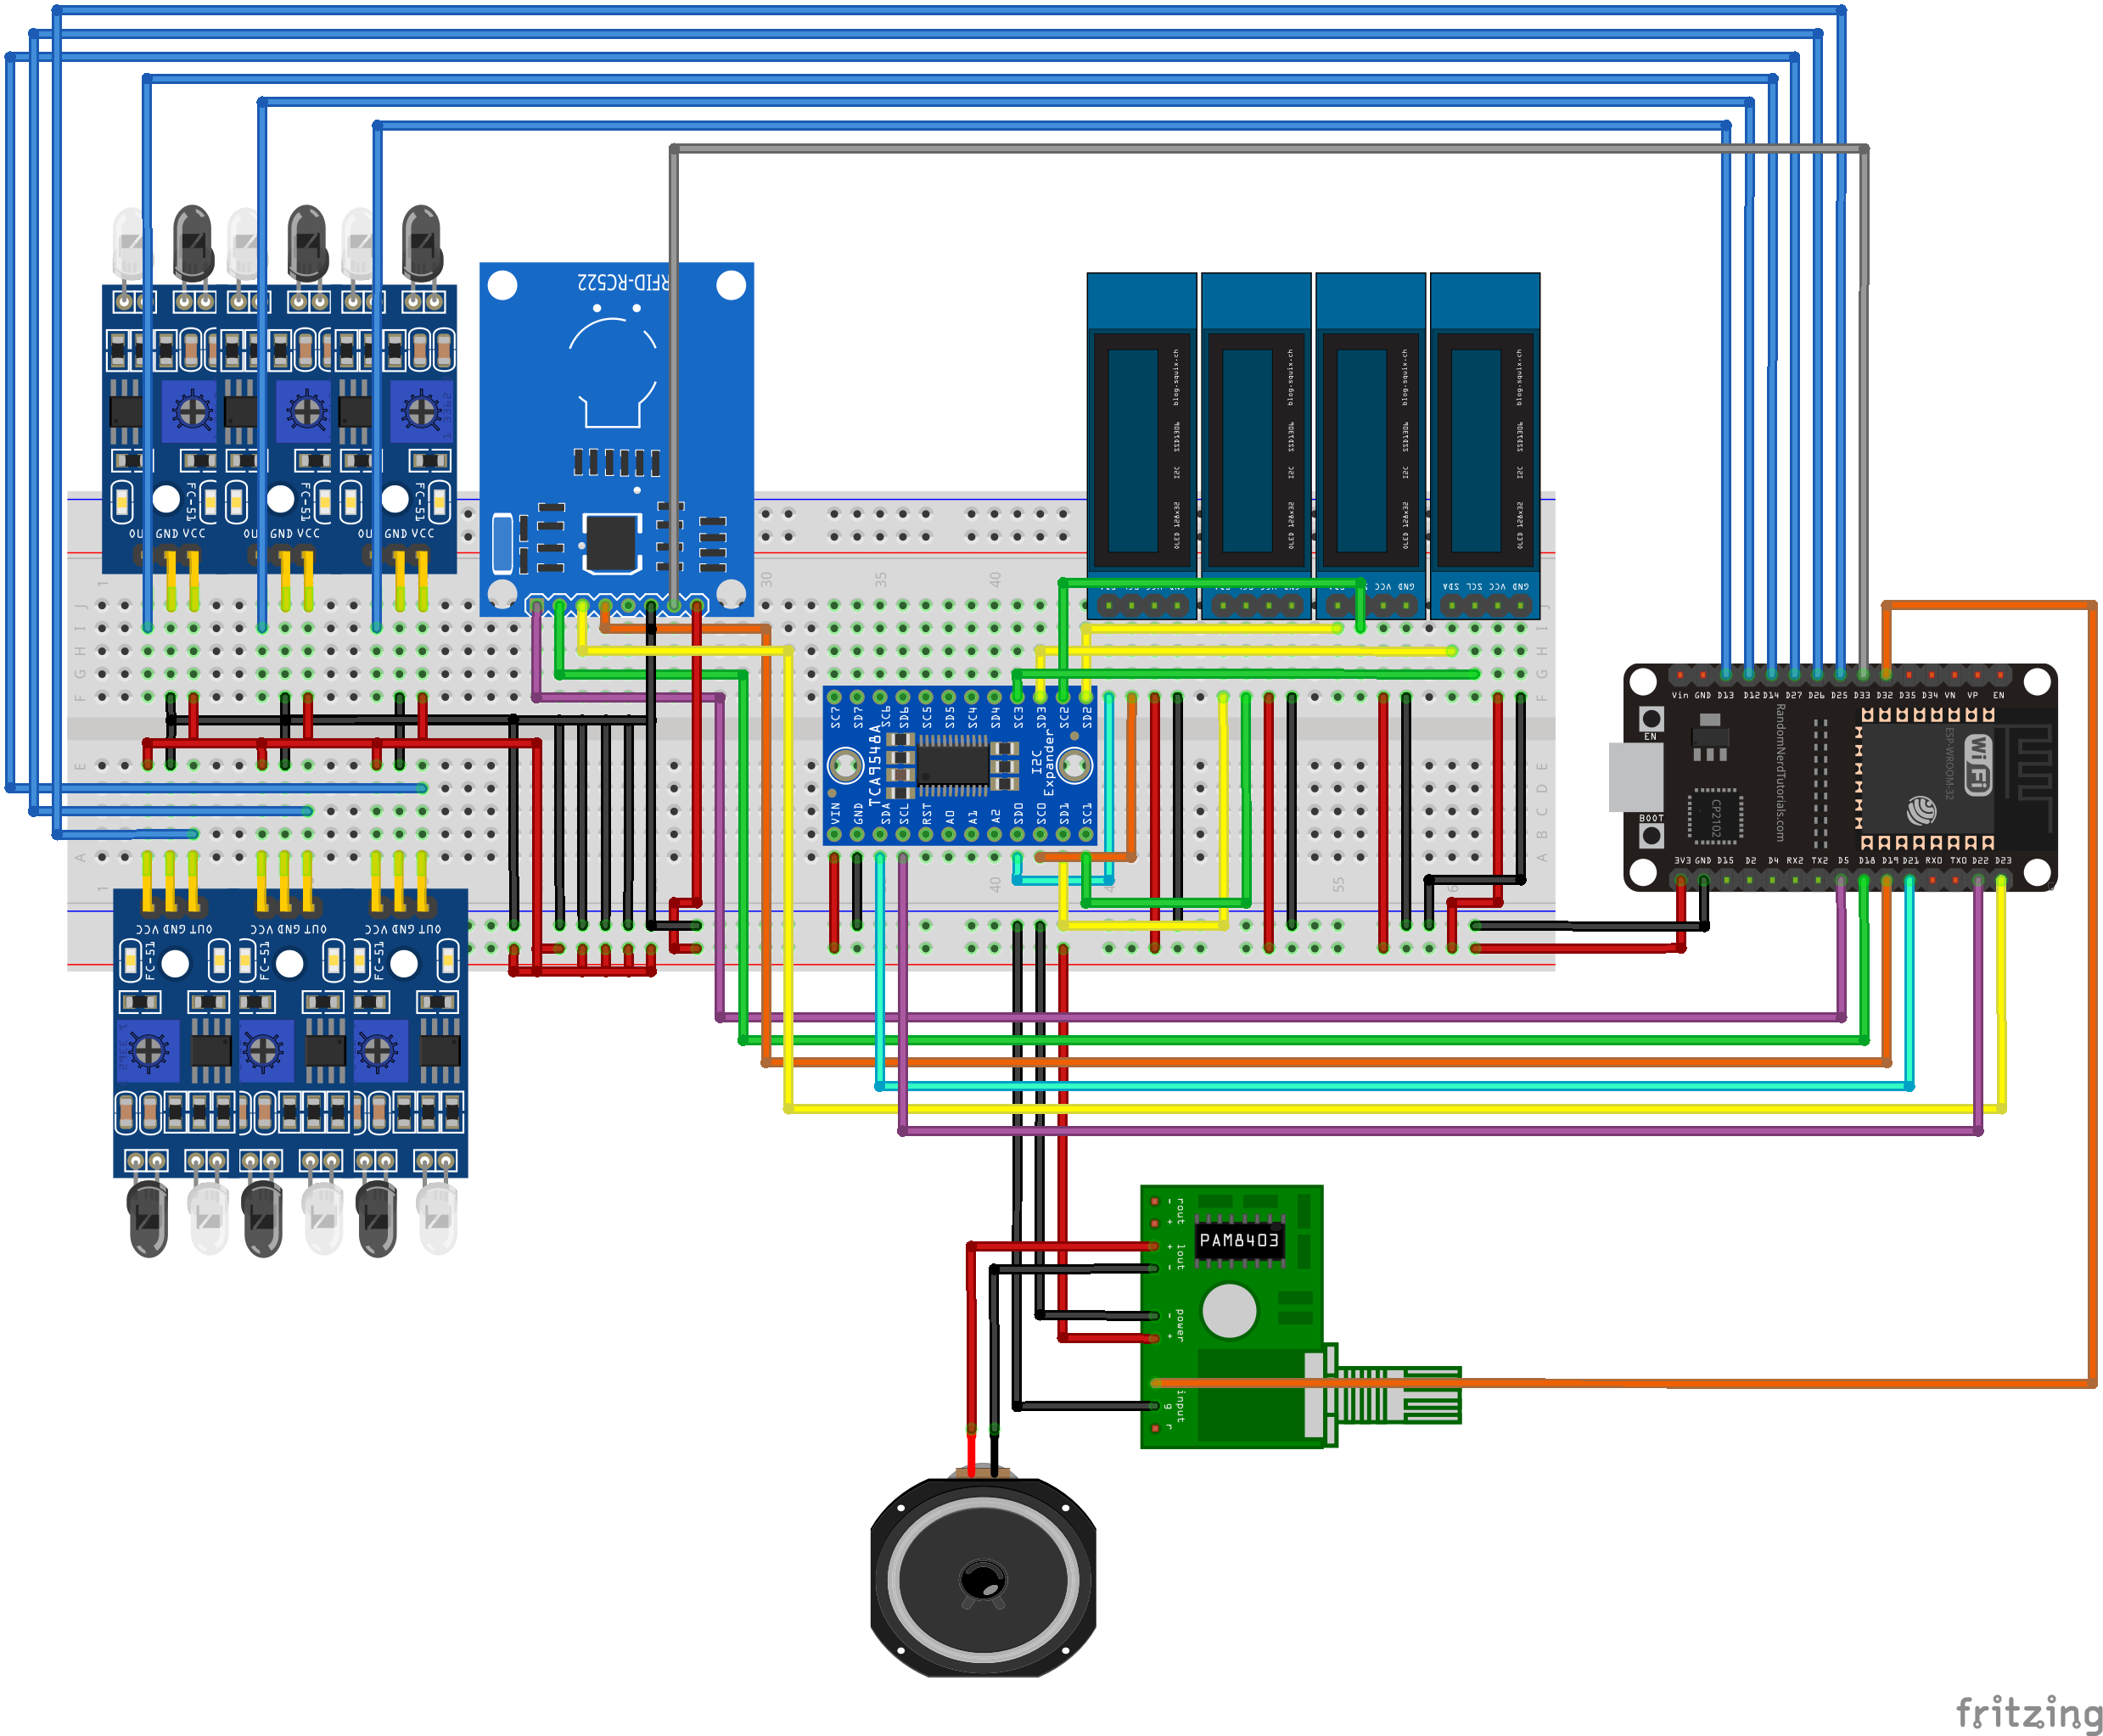
\includegraphics[width=0.9\textwidth]{main_shelf.png}
    \end{center}
    \caption{Electronic Design of main shelf}
    \label{fig:electronics-main}
\end{figure}
\begin{figure}[H]
    \begin{center}
        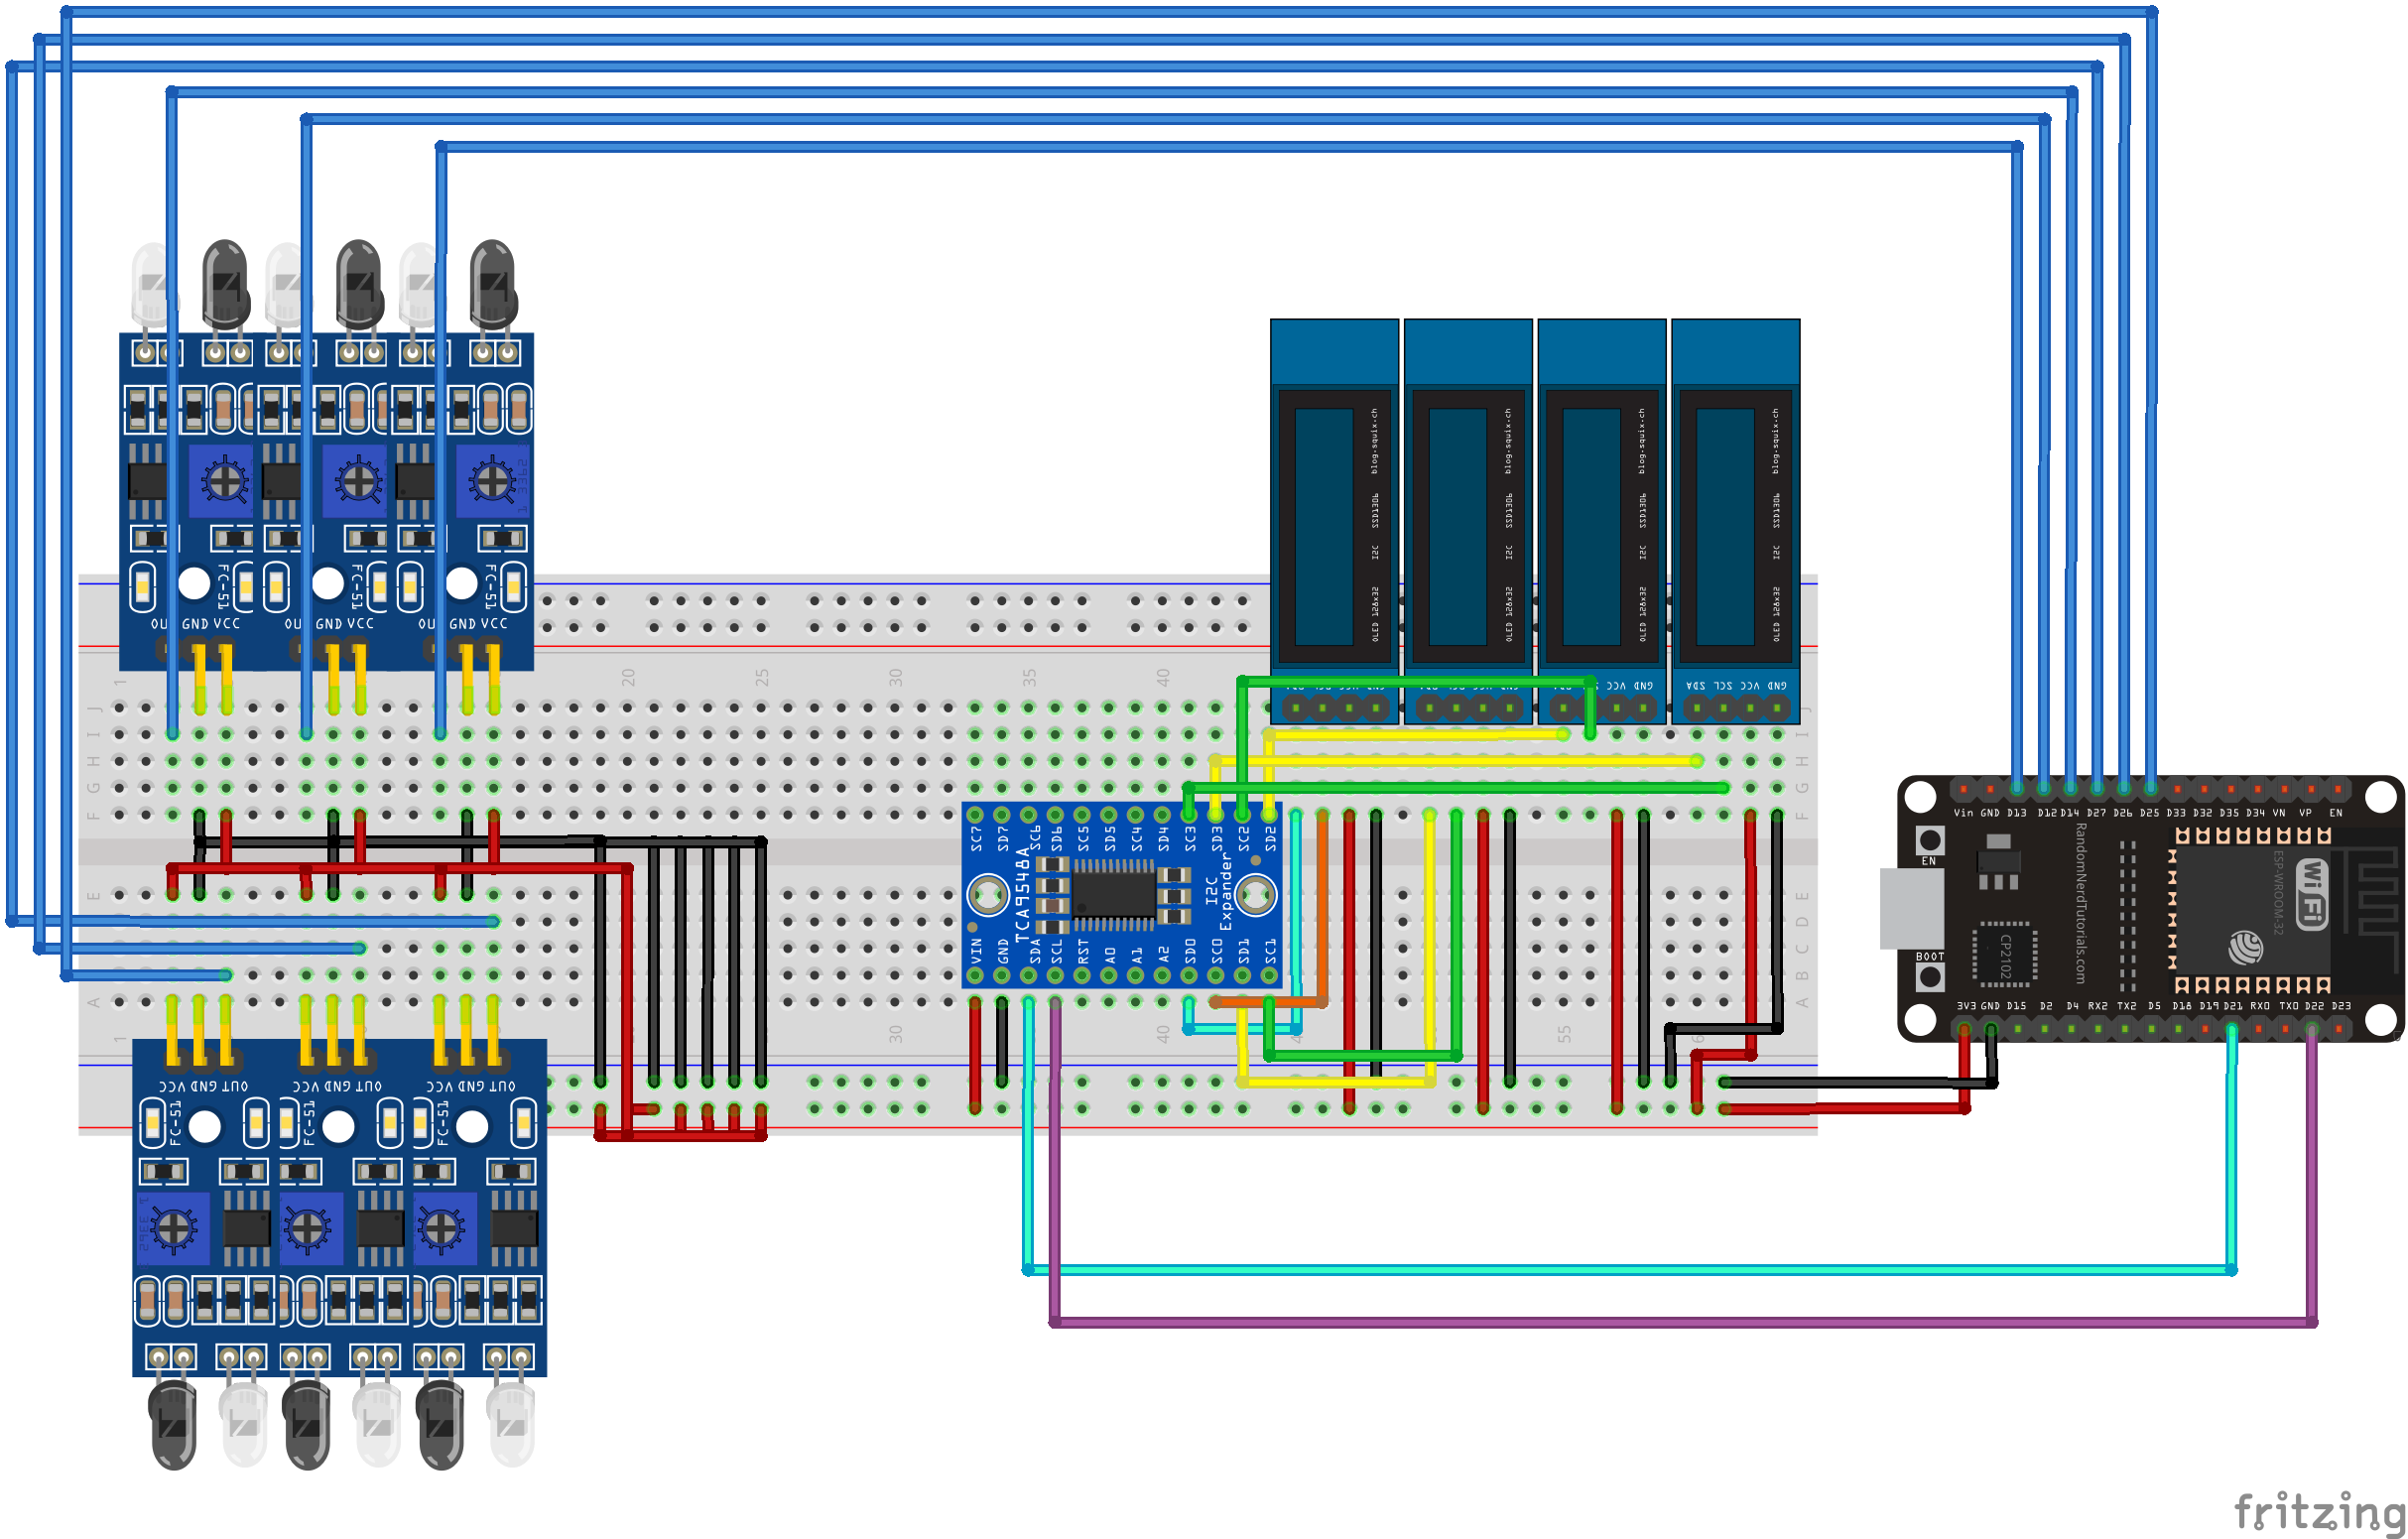
\includegraphics[width=0.9\textwidth]{extension_shelf.png}
    \end{center}
    \caption{Electronic Design of extension shelf}
    \label{fig:electronics-extension}
\end{figure}


\section{Software Design}
For our project we use GitLab to track changes of software development and to manage our code easily. 

The software used in this project is divided into three parts: back end, front end and microcontroller code. The back end is responsible for storing the information in a database and communicating this information to both the user application and the microcontroller on requests. The front end application is created for more convenient wall hangers' and trips' information manipulation by users. The last part is the microcontroller project, which is an Arduino C++ code uploaded to ESP32 WROOM microcontroller to manipulate the hardware parts on the wall hanger according to the user needs.

The full code can be found in \textbf{\href{https://gitlab.science.ru.nl/ndl1/21-22-project/A4}{GitLab}} project and report covers the most important parts and approaches of the project.

\subsection{Back end}
The back end project is created to support both the front end and the microcontroller. It is used to store the configuration of the shelves and trips in the database, to process the information and to provide it to the ESP32 board and front end application on requests. 

We use C\# language and .NET Core framework for programming the application. We use Entity Framework Core data access technology \cite{EFC} to request from and save data to the database. Entity Framework Core is also responsible for managing users and roles and for encoding of vulnerable information such as passwords. We use MS SQL local (relational) database technology for our application and IIS Express server \cite{iis}, which is built in to the Visual Studio, to host it locally on our computers. 

The purpose of the back end application is accessing data in the database, processing it to the format that is acceptable by front end or microcontroller and communicating processed data to the requesting parties. Requests and responses use RESTful Web API methods \cite{REST} and the data is sent in JSON format \cite{JSON}.

The solution consists of 4 projects:
\begin{enumerate}
    \item \textit{Domain} - contains classes that represent database entities (objects);
    \item \textit{DAL} (Data Access Layer) - contains classes that are responsible for accessing database and requesting/saving information to and from the database;
    \item \textit{Identity} - contains helper functions that are creating and reading JSON Web Token (JWT) that is used to identify the user when user-specific information is accessed;
    \item \textit{ShelfWebApp} - the main communication point for REST API and contains application Startup class and API controllers, which process HTTP(S) requests and send responses containing asked information or error description.
\end{enumerate}


\subsubsection{Back end setup and run}
We have used Visual Studio 2019 Community to code and host the back end. The Community version can be downloaded \href{https://visualstudio.microsoft.com/vs/community/}{here}, however, only the VS 2022 version is currently available, while we have used 2019 version of Visual Studio. After Visual Studio is installed it is necessary to add two packages using VS installer: \textit{ASP.NET and web development} and \textit{Desktop development with C++}.

After everything is installed, the back end solution can be opened using \textit{SmartShelf.sln} file, which opens all the projects described in this sub-section. \textit{ShelfWebApp} project should be selected as a start-up project in solution properties and the IIS Express server should be executed. 

The app will not work without a database, so the database should be updated using \textit{Update-Database} command in \textit{NuGet Package Manager $\rightarrow$ Console} (this can be found in VS under \textit{Tools}). It is necessary to select \textit{DAL} as the default project in the console view before executing the update command. 

When the app is executed, it will automatically run on localhost (the port can differ per computer). Our project requires the connection to the back end externally from microcontrollers or if front end is hosted on another computer. For that the IIS Express configuration should be changed to the following: 
\begin{lstlisting}
<binding protocol="http" bindingInformation="*:11226:localhost" />
<binding protocol="https" bindingInformation="*:44315:localhost" />
<binding protocol="http" bindingInformation="*:11226:*" />
<binding protocol="https" bindingInformation="*:44315:*" />
\end{lstlisting}

The first two lines already exist, however, last two lines were added by us and they make possible to run application on the local network (\href{https://mrfields.net/iis-remote-access/}{link to guide}). The IIS Express configuration file is located for us in the following location \textit{SmartShelf-back-end\textbackslash.vs\textbackslash SmartShelf\textbackslash config} and is called \textit{applicationhost.config}. The \textit{.vs} folder appears after the code is built by Visual Studio. After that Visual Studio should be run as administrator. Moreover, the Windows Defender Firewall should also be disabled and it can be done through Control Panel. 
% you might want to add that visual studio should be run as an administrator

When the application is started the database is automatically updated with the categories we defined, however, all wall hangers and trips should be added by users.

\subsection{Front end}
The front end is an application used by an user to add trips and customize their wall hangers, which will then be send to the back end. This will be programmed using the Ionic framework using Vue\cite{ION}. We chose this framework because it has good documentation and is said be easy to learn. Moreover, we use Progressive Web App (PWA) technology, which helps us to create web and mobile applications at once.

\subsubsection{Router}
The router will be used to direct the user to the different pages. The router also checks if user is authorized to access certain pages. For example, if user is not logged in, then they are only allowed to access home page, but the router will automatically redirect to \hyperref[sec:Login]{Login/Register page}.

\subsubsection{Login/Register}
\label{sec:Login}
The user has to login or register to access the rest of the application. This is done by entering login/registration information, which is then posted to the back end which that returns a JSON Web Token (JWT)\cite{JWT}. The JWT is stored using the \textit{auth.js}. This JWT allows the user to access other front end pages and is added to all HTTP(S) requests for user authentication. \hyperref[fig:login]{Figure 9} and \hyperref[fig:register]{Figure 10} show the templates used for login/register pages.

\begin{figure}[H]
    \begin{center}
        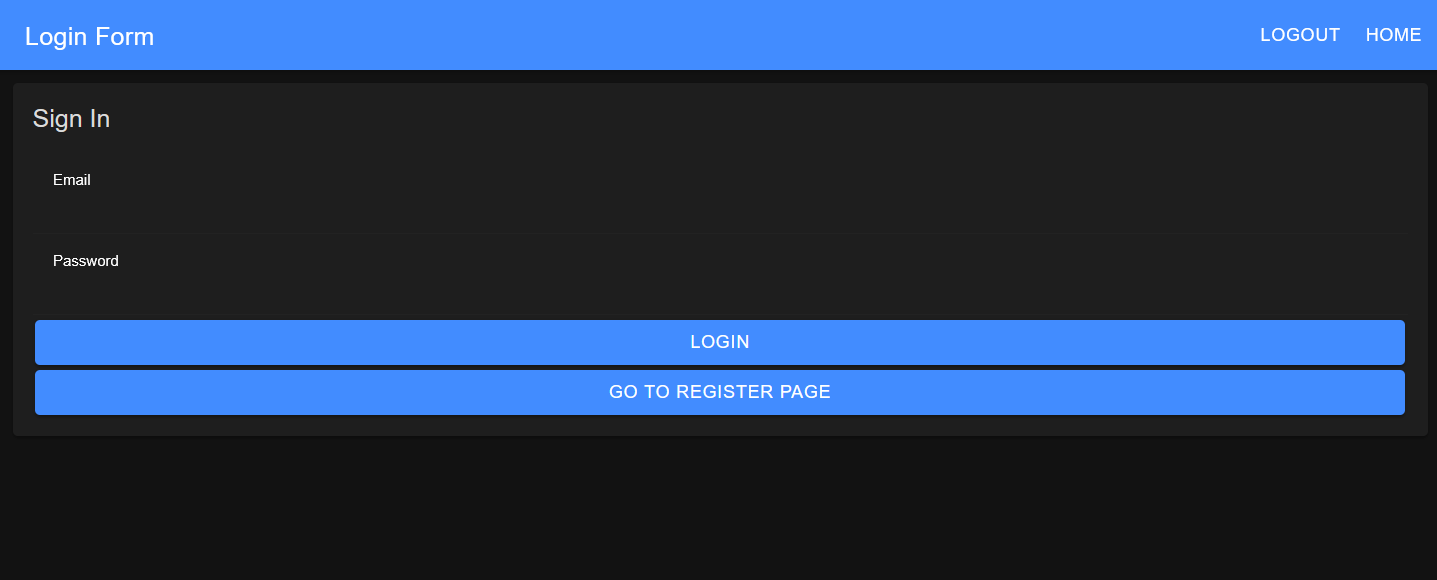
\includegraphics[width=1\textwidth]{Front-End/Login.png}
    \end{center}
    \caption{Login page}
    \label{fig:login}
\end{figure}
\begin{figure}[H]
    \begin{center}
        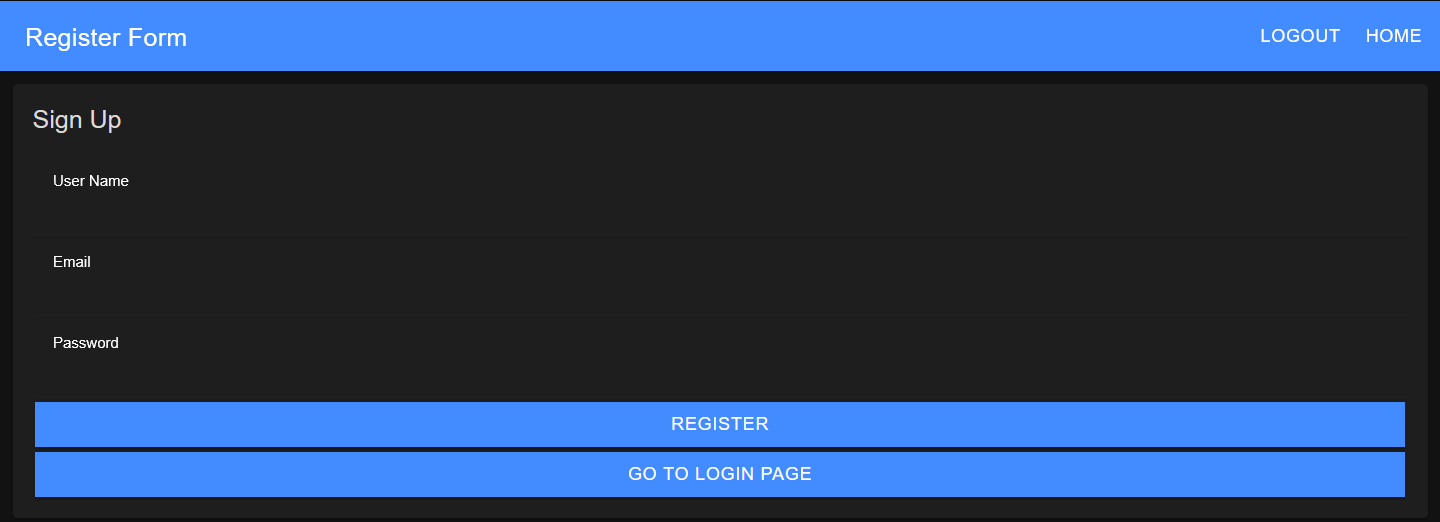
\includegraphics[width=1\textwidth]{Front-End/Register.png}
    \end{center}
    \caption{Register page}
    \label{fig:register}
\end{figure}

\subsubsection{Home Page}
Once the user is logged in, they are redirected to the home page. The home page contains an overview of all their shelves and trips. They can also navigate to other pages to add, edit or delete shelves and trips from the home page. \hyperref[fig:home]{Figure 11} shows the templates of home page.

\begin{figure}[H]
    \begin{center}
        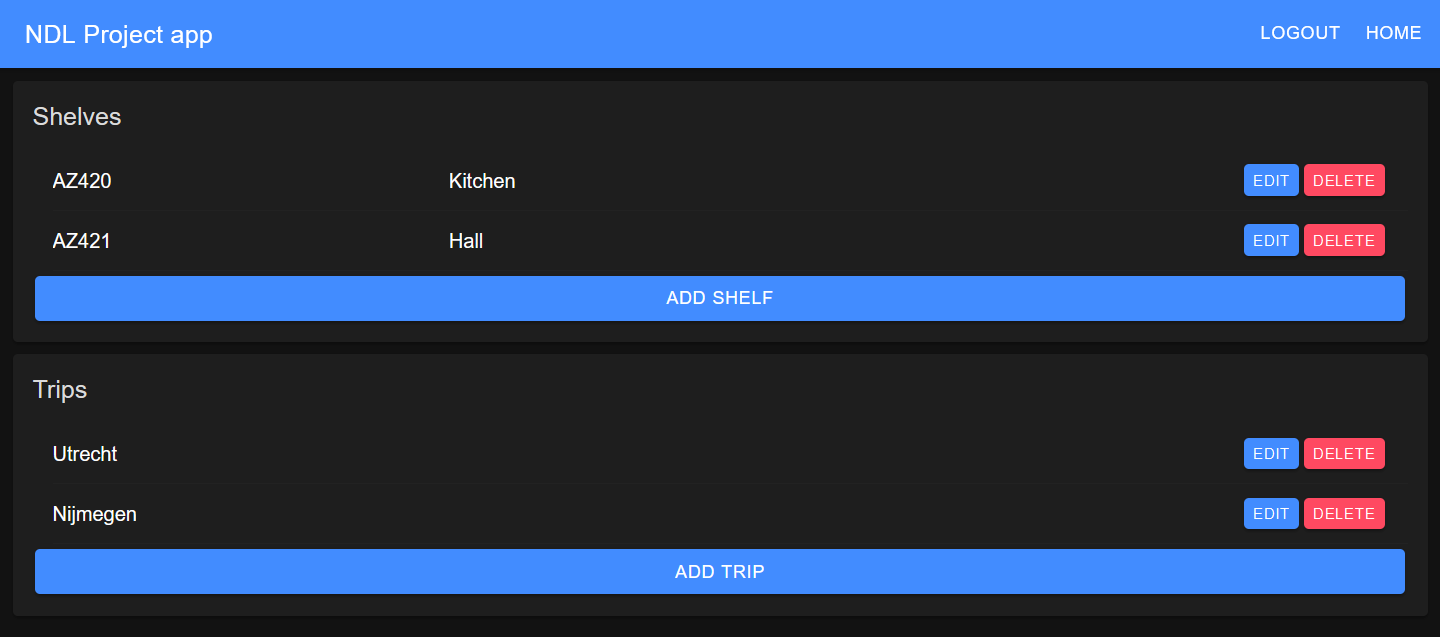
\includegraphics[width=1\textwidth]{Front-End/Main.png}
    \end{center}
    \caption{Home page}
    \label{fig:home}
\end{figure}

\subsubsection{Adding/editing shelves}
\hyperref[fig:add-shelf]{Figure 12} represents the templates of shelf information management. When adding shelves to user's profile they are asked to fill in the identifier of the shelf, if it is a main shelf or not and where the shelf is located. If the shelf is not main, but an extension, the user also has to give the identifier of the main shelf they want to couple it with. This information is then sent to the back end along with user's JWT. In case shelf is being edited, information in the fields is pre-filled for the user on the page load.

\begin{figure}[H]
    \begin{center}
        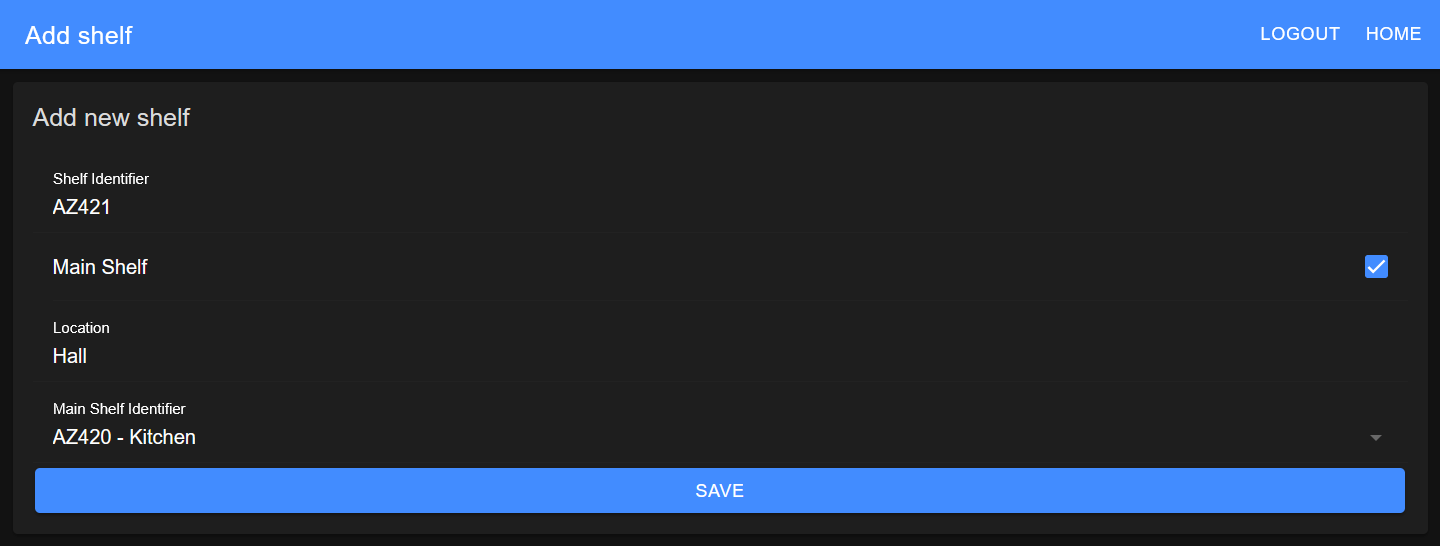
\includegraphics[width=1\textwidth]{Front-End/Shelf.png}
    \end{center}
    \caption{Add/edit shelf page}
    \label{fig:add-shelf}
\end{figure}

\subsubsection{Adding/editing trips}
\hyperref[fig:add-trip]{Figure 13} represents the templates of trip information management. To add a new trip the user has to fill in destination, start- and end-time, reminder time, and for each shelf information about the items they want to take with them on that trip. This information is then sent to the back end along with user's JWT. In case a trip is being edited, information in the fields is pre-filled for the user on the page load. We could not get the editing of trips to work properly  due to reasons we discuss in \hyperref[sec:front]{Front end problems} section.
\begin{figure}[H]
    \begin{center}
        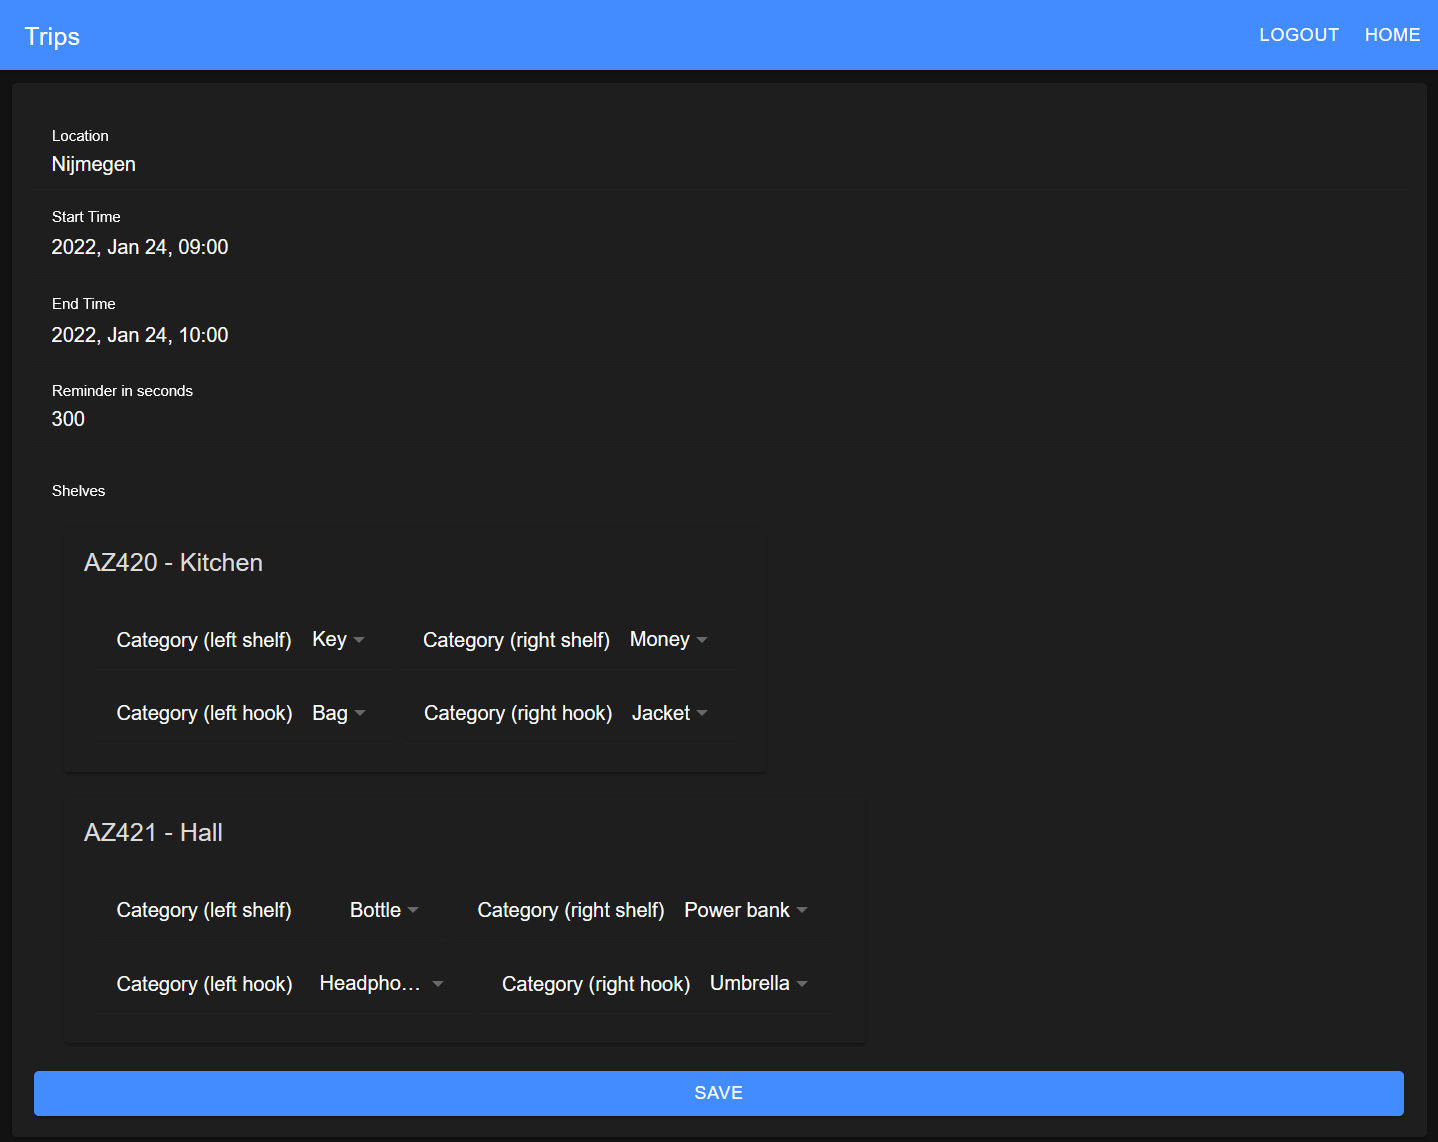
\includegraphics[width=1\textwidth]{Front-End/Trips.png}
    \end{center}
    \caption{Add/edit trip page}
    \label{fig:add-trip}
\end{figure}

\subsubsection{Front end setup and run}
To run the front end it is necessary to install the Ionic client, First, Node.js and npm should be installed. To verify this the following commands should return the version number:
\begin{lstlisting}
$ node --version
$ npm --version
\end{lstlisting}

If they are not installed following the   \href{https://ionicframework.com/docs/intro/environment}{instructions here} will help with this step.

Once Node.js and npm are installed, the following command can be used to install the Ionic client:
\begin{lstlisting}
$ npm install -g @ionic/cli
\end{lstlisting}
Once this is done, go to the directory where the front end is located (in our case the /front-end folder) and enter the following command in your terminal:
\begin{lstlisting}
$ ionic serve
\end{lstlisting}
If any problems are encountered during the installation, please refer to their installation guide \href{https://ionicframework.com/docs/intro/cli}{here}.\cite{IONIN}

To get the communication with the back end work, it might be necessary to edit the URL in the \textit{URL.js} file, which can be found in the \textit{/front-end/src/store/modules} folder. The URL of back end can be found when back end is executed and typical ports for us were port 44315 for HTTPS and port 11226 for HTTP.

\subsection{Arduino code}
We use Arduino ESP32 WROOM as a microcontroller to connect all the hardware parts. \hyperref[fig:electronics-main]{Figure 7} and \hyperref[fig:electronics-extension]{Figure 8} represent how Arduino is integrated in the project along with other hardware components. Its purpose is to communicate with the back end and configure other hardware components according to the data it received. 

It starts with fetching the information of the next trip, which contains the start time, reminder time (optional) and screen configurations. It processes this information and starts with updating screens with the logo and text of the corresponding items` categories. When the current date and time is equal to the reminder time, it plays \textit{Pirates of the Caribbean} themed melody to notify user about the time to leave or to prepare for leaving. The user decides themselves what meaning they give to the set reminder. Starting an hour before the trip start time it is possible to check out using NFC tag, which means that user has left the house, and then the shelf configuration is updated with the configuration of the following trip. IR obstacle sensors detect if items are placed or removed from the hooks/shelf sections and information regarding that is updated with the back end. 

\subsubsection{Arduino libraries}
In addition to the code we wrote ourselves, we also used some external drivers and libraries that are listed below: 
\begin{itemize}
    \item U8g2 by oliver \cite{u8g2} 
    \item MFRC522 by GithubCommunity \cite{MFRC522}
    \item HttpClient by Adrian McEwen \cite{httpclient}
    \item ESP8266-OLED Display Library by Klar Systems \cite{esp-oled}
    \item ESP8266 and ESP32 OLED driver for SSD1306 displays by ThingPulse \cite{oled-driver}
    \item ArduinoJson by Benoit Blanchon \cite{arduino-json}
    \item WIFI by Arduino \cite{wifi}
    \item NTPClient by Fabrice Weinberg \cite{ntpclient}
\end{itemize}
It is necessary that the correct board installed in the Arduino IDE by adding this link \href{https://dl.espressif.com/dl/package_esp32_index.json}{\text{https://dl.espressif.com/dl/package\_esp32\_index.json}} to the preferences in the additional boards manager URL field. \textit{"ESP32 Dev Module"} should be selected in tools.

\section{Usage guide}
The user starts with getting the shelves. The user registers in the application and logs in. They start with adding main wall hangers (shelves) and continue with extension wall hangers addition. The main identification, which the user enters when adding shelf, for the wall hangers is hard-coded in Arduino identification code that is globally unique for all our shelves. This code is used for requesting wall hanger specific information from the back end. When all shelves are added (should be at least one) it is possible to add planned trips. The user adds location, start and end date and time, reminder time and shelves configuration with corresponding categories of items that user has to take with them. When this information is saved, the corresponding wall hanger requests it from the back end. It receives the soonest trip information, displays selected item categories on the OLED screens and speaker goes off when it is a reminder time. NFC tag is used to check out when user leaves the house.

\section{Pitfalls}
We have encountered some difficulties in our project that we did not expect to have when we were planning this project. These difficulties are covered in this section.

\subsection{IR sensors} 
\label{sec:ir}
We ran into a few problems with our IR sensors. Some of the solutions we found are not perfect, however, we implemented them due to the time restrictions we had.

\subsubsection{Poor design}
The first problem we ran into was that some of our IR sensors were not working correctly, they seemed to always return that there was an object detected. After some time we found the cause of the problem: the LED would shine directly into the sensor instead of bouncing of a surface at first. We were able to fix it by putting some heat shrink around the LEDs, which prevented it from shining directly into the sensor.

\subsubsection{Sensitivity of the sensor}
The other problem we encountered was that sensors detected the shelf/hook instead of the item on it. We were able to fix it by using some black tape to cover hooks/shelves and eliminate reflection. The grey hooks printed later did not have this problem.

\subsection{3D models decisions problems} 
\label{sec:3dproblems}
To begin with, our screen holder design in \hyperref[fig:screen]{Figure 2} had some drawbacks we discovered during the assembly. Firstly, the space between middle part that keeps screen in place and holes designed for attachment to the wood is too small to make it possible to screw the holder to the wood. Thus, we used glue for attachment. Secondly, we did not have tools to make space in the wood for wires going from the holders to the controller located one the top of the shelf. Ideally we would have made a recess for wires in the back panel between the screen holder and the shelf and they would have been connected to the Arduino through the hole on the back of detail we showed in \hyperref[fig:shelf-back]{Figure 4}. But instead we taped wires to the front and side parts of the wood and, thus, the design did not fully correspond to what we ended up with.

\subsection{Front end problems}
\label{sec:front}
We encountered a few problems with the front end, for one we could not find a reliable way to display the values that were previously assigned to a shelf/trip into the drop down menus, which makes editing shelves/trips less intuitive. Besides that, we could not get editing trips to work because of the previous issue.

\newpage

\section{Conclusion}
We were able to implement most of the features that we wanted to implement. The shelves are modular and can be configured by the user using the front end. But some extra features we were not able to implement like a notification system to the front end and being able to edit trips. With some extra time this would probably have been possible.

The start of the project took quite some time. We started with back end development and coding hardware pieces separately. For each piece we found corresponding library and made it work as we wanted to. Designing of the screen views and designing of the 3D pieces also took quite some time: for the screens we had to find/make logos and design texts, making all the 3D models also required some work with \href{https://www.tinkercad.com}{Tinkercad}. This part of the project gave us quite handy experience for creating personalized details, when there is no market to suggest details that are required for idea implementation, like our project.

IR obstacle sensor problems we described in pitfalls \hyperref[sec:ir]{IR sensors} section took some hours to figure out what caused them and solutions to fix them, because their cause were not intuitive in most of the cases and required code check and experimenting. Other hardware parts we were working with were less problematic and mostly required only some coding. 

We only really started working on the front end part towards the end of the course and during the Christmas break, however, due to the lack of knowledge and experience with VueJS the work was slow and required a lot of searching for the correct way of writing the application. Such lack of experience and time for finishing the project caused such missing front end, where only necessary functionality was implemented, but some more detailed features were only partially implemented. For example, missing functionality for sending a notification about forgotten items (IR sensors detect items that are still present on hook/shelf section) can be solved using SignalR \cite{signalr}.

In conclusion, we think that most important features such as adding shelves and trips and notifying users about the items they need to take with them and when they need to leave were implemented well. We are still missing some nice features, however, their absence does not affect usability of the wall hangers in a mayor way and they can still be a nice addition to the entrance of the user's apartment.

\newpage

\bibliographystyle{plain}
\bibliography{refs}

% \section{Logbook}
% In this section we will describe the process of working on our project by weeks, showing our progress.

% \subsection{1st week: 20.09-26.09}
% First week was project introduction and wish list creation week.\\
% During the first lab class we have presented out project to the audience and listened to the other project ideas. Initially we planned to use other components, but after getting the feedback we considered the following changes:
% \begin{itemize}
%     \item Instead of LED lights we now considered using OLED screens, which makes our system more complex and allows used to change the categories shown on the screens;
%     \item We decided to add item detection to our solution, which will detect items placed on hooks and shelves. For this we decided to use IR obstacle detection sensors;
%     \item Button in our project was replaced with NFC reader. Using NFC reader the user will notify our system that they have left and there is no need for trip reminder. 
% \end{itemize}
% During the end of the first and during the second lab class this week we spent time on searching for the components and engineering the way we were going to place them on the shelves. 

% \subsection{2nd week: 27.09-03.10}
% This week we fully focused on the software we will use for our smart-shelf support. We started with creating front-end and back-end of the application we are planning to use to manage our shelves. Through the application users will add their trips, will select where and what time they will be and select the categories of items they plan to take. \\
% We started with creating a database schema, working in parallel on front-end understanding and the UI creation. After the database schema was ready we continued with developing the app itself, adding user management and REST API to our application. We also tried to host the app from one computer and connect to it from another, which was possible when changing IIS Express configuration, turning off Windows Firewall and using local network for connection.

% \subsection{3rd week: 04.10-10.10}
% This week we decided to stop working on the software and worked a bit on a hardware part: mostly on understanding how the components we are going to use work. We tried to connect multiple screens using I2C multiplexer and figured out how to work with them. Moreover, we tried to connect the speaker and amplifier, which took some time, because we could not quickly find connection schema on the Internet. We managed to connect it and play some sounds, but we decided to leave it for the end, because the speaker was too loud and disturbing other people. At the end of the week we printed some durable hooks and tried IR sensors on them. However, sensors were malfunctioning and were not detecting objects properly and these were our assumption of what could go wrong: they were facing too down and reflecting from the bottom of the hook; they were placed too up and did not detect objects placed to the bottom; the surface of the hook is too reflective and IR light reflects in different direction.

% \subsection{4th week: 11.10-17.10}
% This week some more parts were delivered, we finally got our esp-32 wroom's and displays and some more IR sensors. We started with trying out how the new displays worked and started making the icons and text to display on them. Then we worked on trying to get them to work with the multiplexer, so we could show different items on each display.

% \subsection{5th week: 18.10-24.10}
% This week we started working on testing the new IR sensors since they are a different model then the once we used before, we had some trouble getting them to work but after some time we found the problem. The IR led was shining straight into the sensor so it would always be turned on so we put some heat shrink on the LED's to fix this. We also finally got the displays to display the correct icons and text etc. We also updated the hooks so that we could screw the IR sensor onto the hook. After this we started trying to get the NFC reader to work to no avail. We also started working on trying to connect the ESP to the back-end and updated the back-end some more. And lastly we also sawed the wood.

% %monday: ir sensors again, didnt work, multiplexer with screens to dispaly different things, updating hooks

% %thursday: sawing the wood, trying nfc, working on back end, starting with trying to connect esp to backend and figure out how json works on arduino.

% \subsection{6th week: 8.11-14.11}


\end{document}
